\documentclass[tikz,border=3mm]{standalone}
\usetikzlibrary{arrows.meta, positioning, shapes.geometric}
\usepackage{fontspec}
\setmainfont{Roboto}

\definecolor{cvutblue}{cmyk}{1, 0.43, 0, 0}

\begin{document}
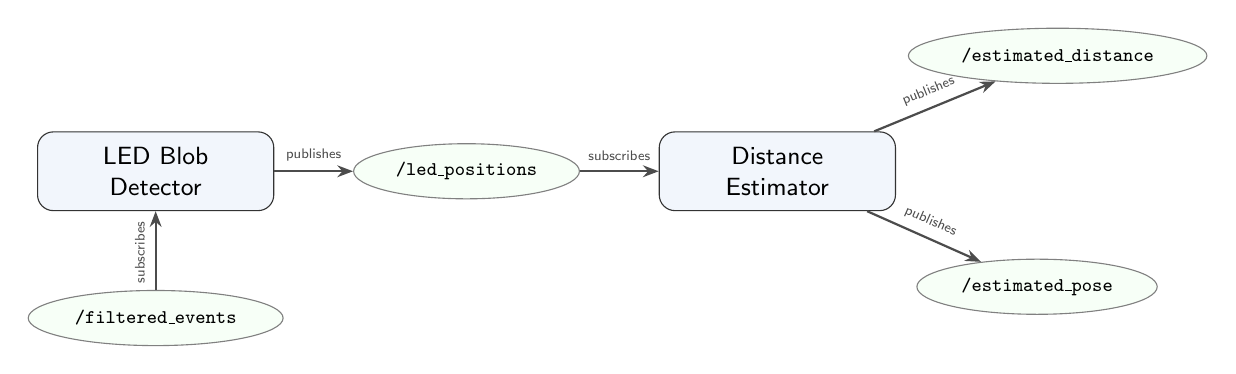
\begin{tikzpicture}[
    node distance=10mm,
    block/.style={
        rectangle, 
        rounded corners=2mm, 
        draw=black!80,
        fill=cvutblue!5,
        minimum width=3cm,
        minimum height=1cm,
        align=center,
        font=\small\sffamily
    },
    topic/.style={
        ellipse,
        draw=black!50,
        fill=green!3,
        minimum width=2cm,
        minimum height=0.7cm,
        align=center,
        font=\scriptsize\ttfamily
    },
    arrow/.style={
        -{Stealth[length=2mm]},
        thick,
        black!70
    },
    label/.style={
        font=\tiny\sffamily,
        above,
        sloped
    }
]

\node[block] (detector) {LED Blob\\Detector};
\node[topic, right=of detector] (positions) {/led\_positions};
\node[block, right=of positions] (estimator) {Distance\\Estimator};
\node[topic, above right=of estimator] (distance) {/estimated\_distance};
\node[topic, below right=of estimator] (pose) {/estimated\_pose};

\node[topic, below=of detector] (filtered) {/filtered\_events};

\draw[arrow] (detector) -- (positions) node[label,midway] {publishes};
\draw[arrow] (positions) -- (estimator) node[label,midway] {subscribes};
\draw[arrow] (estimator) -- (distance) node[label,midway] {publishes};
\draw[arrow] (estimator) -- (pose) node[label,midway] {publishes};

\draw[arrow] (filtered) -- (detector) 
    node[label,pos=1.2,left,xshift=-2mm,yshift=2mm] {subscribes};

\end{tikzpicture}
\end{document}